% !TEX program = xelatex
% 中心科学实验 IV 研究型实验报告模板
% 化学国家级实验教学示范中心（厦门大学）

\documentclass[a4paper]{article}

% ===== 字体 =====
\usepackage{fontspec}
\usepackage{xeCJK}
\setCJKmainfont[BoldFont=SimHei]{SimSun}      % \textbf 中文 → 黑体
\setCJKsansfont[BoldFont=SimHei]{SimHei}
\setCJKmonofont{FangSong}
\newCJKfontfamily\heiti[BoldFont=SimHei]{SimHei}
\newCJKfontfamily\kaishu{KaiTi}
\newCJKfontfamily\fangsong{FangSong}
\newCJKfontfamily\xingkai{STXingkai}
% 开启假粗体后备（对没有显式 BoldFont 的字体合成加粗）
\xeCJKsetup{AutoFakeBold=true}
\setmainfont{Times New Roman}

% ===== 字号定义 =====
\newcommand{\zihaoSan}{\fontsize{16pt}{24pt}\selectfont}
\newcommand{\zihaoSi}{\fontsize{14pt}{21pt}\selectfont}
\newcommand{\zihaoWu}{\fontsize{10.5pt}{16pt}\selectfont}
\newcommand{\zihaoXiaoWu}{\fontsize{9pt}{13.5pt}\selectfont}
\newcommand{\zihaoLiu}{\fontsize{7.5pt}{11pt}\selectfont}

% ===== 正文行距 =====
% 10.5pt字体，行距16pt，linespread=16/(10.5*1.2)=1.2698
\usepackage{setspace}

% ===== 页面 =====
\usepackage[a4paper,
  top=4.6cm, bottom=3.0cm,
  left=2.5cm, right=2.0cm,
  headheight=3.8cm,
  headsep=0.8cm,
  footskip=1.8cm]{geometry}

% ===== 页眉页脚 =====
\usepackage{fancyhdr}
\usepackage{graphicx}

\newcommand{\infobar}{%
  \zihaoWu
  \setlength{\tabcolsep}{0pt}%
  \vspace{0.5em}
  \begin{tabular}{@{}p{0.315\textwidth}p{0.315\textwidth}p{0.315\textwidth}@{}}
    系（Dept.）\underline{\hspace{2.2cm}} &
    专业（Major）\underline{\hspace{1.3cm}} &
    学号（ID）\underline{\hspace{1.3cm}} \\[7pt]
    姓名（Name）\underline{\hspace{1.6cm}} &
    日期（Date）\underline{\hspace{1.5cm}} &
    实验台号（No.）\underline{\hspace{0.8cm}}
  \end{tabular}%
  \vspace{1em}
}

\newcommand{\myhead}{%
  \begin{minipage}[c]{2cm}%
    
\includegraphics[height=2cm]{images/img-000.png}%
  \end{minipage}%
  \vspace{-0.5em}%
  \begin{minipage}[c]{\dimexpr\textwidth-1.8cm\relax}%
    \centering
    {\hspace{-1.5em}\zihaoSan\heiti 中心科学实验 IV\hspace{2em}{\xingkai 实\kern0.2em 验\kern0.2em 报\kern0.2em 告}}\\[3pt]
    {\hspace{-1.5em}\fontsize{11pt}{14pt}\selectfont\textbf{Experimental Report of Central Science}}\\[6pt]
    \infobar
  \end{minipage}%
}

\pagestyle{fancy}
\fancyhf{}
\renewcommand{\headrulewidth}{0.4pt}
\renewcommand{\footrulewidth}{0.4pt}
\fancyhead[L]{\myhead}
\fancyfoot[C]{
  \vspace{-0.5em}
  \zihaoWu \bfseries 化学国家级实验教学示范中心（厦门大学）\\[1pt]
  {\textbf{\fontsize{9pt}{13pt}\selectfont
    National Demonstration Center for Experimental Chemistry Education (Xiamen University)}}
}

\fancypagestyle{plain}{%
  \fancyhf{}
  \renewcommand{\headrulewidth}{0.4pt}
  \renewcommand{\footrulewidth}{0.4pt}
  \fancyhead[L]{\myhead}
  \fancyfoot[C]{
    \vspace{-0.5em}
    \zihaoWu \bfseries 化学国家级实验教学示范中心（厦门大学）\\[1pt]
    {\textbf{\fontsize{9pt}{13pt}\selectfont
      National Demonstration Center for Experimental Chemistry Education (Xiamen University)}}
  }
}

% ===== 标题样式 =====
\usepackage{titlesec}
\titleformat{\section}{\zihaoSi\heiti}{\thesection}{1em}{}
\titlespacing{\section}{0pt}{12pt}{6pt}
\titleformat{\subsection}{\zihaoWu\heiti\bfseries}{\thesubsection}{1em}{}
\titlespacing{\subsection}{0pt}{0pt}{0pt}

% ===== 表格图片 =====
\usepackage{booktabs}
\usepackage{multirow}
\usepackage{caption}
\captionsetup[table]{labelsep=space,font={small},position=above,skip=4pt,justification=centering}
\captionsetup[figure]{labelsep=space,font={small},position=below,skip=4pt,justification=centering}

% ===== 参考文献 =====
\usepackage[super,sort&compress]{natbib}
\bibliographystyle{unsrt}

% ===== 其他 =====
\usepackage[colorlinks=true,linkcolor=black,urlcolor=blue,citecolor=black]{hyperref}
\usepackage{indentfirst}
\setlength{\parindent}{2em}
\setlength{\parskip}{0pt}
\usepackage{enumitem}
\setlist{nosep}

% ======================================================
% 评语与签字栏（整体不分页，置于最末）
\usepackage{needspace}

% ======================================================
\begin{document}

% 全文行距设为 16pt（正文10.5pt对应linespread=1.2698）
\setstretch{1.05}
\zihaoWu

% ===== 题目 =====
\begin{center}
	{\zihaoSan\heiti 题目（3 号黑体，居中）}
\end{center}

\vspace{6pt}

% ======================================================
\section{引言（一级标题为 4 号黑体）}
\vspace{-0.5em}

（正文为 5 号宋体，行间距 16 磅）应阐明本实验的背景、意义，通过图书馆的中国期刊网
\url{http://kns.cnki.net/kns/brief/result.aspx?dbprefix=CJFQ}
或查找相关英文文献 \url{https://scifinder.cas.org}，对国内外有关与本实验相关的研究状况进行较为全面的介绍，
并适当引用文献，尤其是近五年发表的文献。

% ======================================================
\section{实验部分}
\vspace{-0.5em}

\subsection{仪器与试剂（二级标题 5 号黑体）}

仪器和试剂应用中文标明规格或纯度、型号、名称、国别及生产商。

\subsection{实验方法}

应分清层次，可分节给出，并加上适当的小标题。此部分应详细叙述实验方法和实验条件，不要罗列全部实验过程，
只需叙述实验最终确定的主要和关键部分的具体操作步骤、测试条件和仪器参数，以能够使他人重复实验为准。
实验方法如参考自文献，应引用该文献。

% ======================================================
\section{结果与讨论（此处可以按实验内容分点，每个主题有各自的标题，结果分析和图表）}
\vspace{-0.5em}

\subsection{内容（二级标题 5 号黑体）}

此部分为全文的重点。数据是表现结果的重要方式，必要时可用照片、图和表格表示；文字用于对研究结果进行必要的
说明、解释，与他人结果进行比较，阐明本项工作的意义或局限性，突出本研究的新发现及经过证实的新观点、新见解。
同时要探讨所得到的结果与研究目的的关系、是否符合原来的期望、与他人结果的异同比较和分析、结果的意义（推论）。
有些实验结果在某些方面出现异常，无法解释，虽不影响主要论点，但要说明，供其他研究者参考。也可在这一部分提出
本研究存在的难以解决或尚需进一步探索的问题。此部分不能仅仅罗列堆积实验数据或观察事实，应从数据中提炼出有价值
的结论，结合本实验数据和结果并参考有关文献或者标准，进行深入讨论。

\subsection{图表}

为了使图表具有自明性和便于交流，对图和表提出下列要求：

\begin{enumerate}[label=(\arabic*),leftmargin=3em,itemsep=0pt,parsep=0pt,topsep=4pt]
	\item 图表中的图题、表题和表内各项内容、图注、表注需标注清楚，采用三线表格式。
	\item 图题与表题应详细、完整、具体，例如"溶菌酶的活性回收率"这个表题不及"不同色谱条件下溶菌酶的活性回收率"具体。
	\item 在图注和表注中给出主要实验条件，每一图序号下的各个图，以 ABCD 区分，每张图中的曲线，以 abcd 标注，并在图注中明确标示其内容。
	\item 图表中若有缩写词或代号，应在第一次出现的图注或表注中给出中英文全称或解释。
	\item 图表中的非专有名词一般不用缩写。
	\item 图表要避免重复，数目尽量精简。同一来源的数据只需用图或用表表达一次，图表中的数据应与正文和摘要中的相关数据一致。
	      请采用适当的有效数字位数，同一图表中的数据的有效数字应保持一致。
	\item 请提供层次分明的黑白或彩色图片。插图清晰，坐标标度准确标明，横纵坐标的名称和单位应齐全，且标注清楚。
	      不要直接使用仪器提供的图谱，请采用绘图软件重新绘制。图片分辨率应达到 600~dpi 以上。
	      所有图表必须在正文中有所提及，并插入到首次提及的段落后。半栏图大小控制在 50~mm$\times$80~mm，
	      通栏图以宽 150~mm 比例缩放，横纵坐标名称标尺数字采用 6 号，图内数字采用 6 号。
\end{enumerate}

图表示例如下：

\begin{table}[htbp]
	\centering
	\caption{{\zihaoXiaoWu ********* （小 5 号字）}}
	\label{tab:example}
	\scalebox{1.2} {
		{\zihaoLiu
			\begin{tabular}{cccc}
				\toprule
				序号                 & 化合物                               & 离子对（$m/z$） & 碰撞电压（eV） \\
				\midrule
				\multirow{2}{*}{1} & \multirow{2}{*}{（表中文字和数字采用 6 号字）} & 127/65*    & 20       \\
								&                                   & 127/92     & 10       \\[2pt]
				\multirow{2}{*}{2} & \multirow{2}{*}{3-CA, 4-CA}       & 127/65*    & 20       \\
								&                                   & 127/100    & 15       \\[2pt]
				\multirow{2}{*}{3} & \multirow{2}{*}{2,6-DCA}          & 161/90*    & 20       \\[2pt]
								&                                   & 163/90     & 20       \\[2pt]
				\multirow{2}{*}{4} & \multirow{2}{*}{2,4-DCA, 2,5-DCA} & 161/99*    & 20       \\
								&                                   & 161/63     & 30       \\
				\bottomrule
			\end{tabular}
		}
	}
\end{table}

\begin{figure}[htbp]
	\centering
	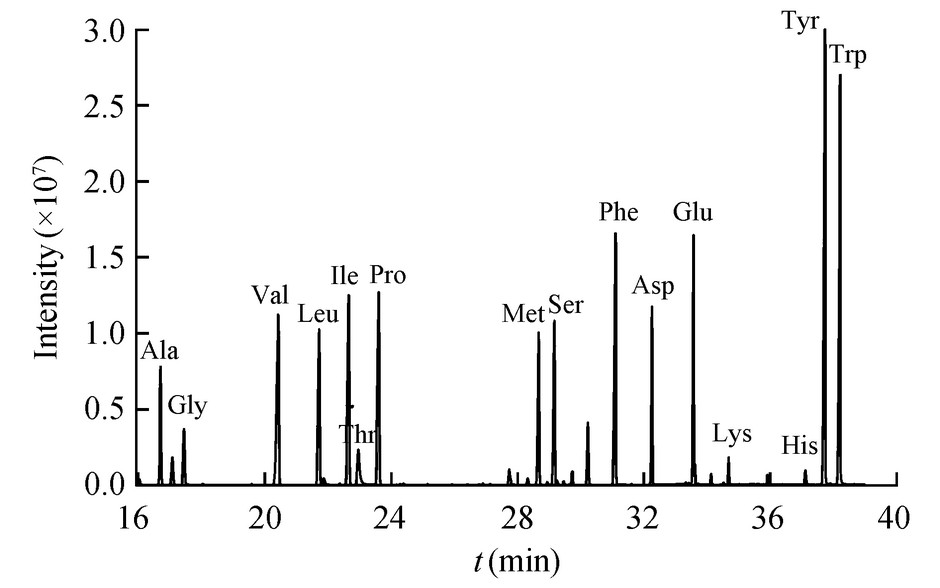
\includegraphics[width=0.6\linewidth]{images/img-001.jpg}
	\caption{{\zihaoWu ********** （5 号字）}}
	\label{fig:example}
\end{figure}

\subsection{物理量、计量单位及其符号}

计量单位及符号必须按《中华人民共和国国家计量标准》及有关 GB 标准规定书写。物理量的符号一律用斜体字母，
单位符号用正体字母。请特别注意浓度单位的表示方法，如不能用 ppm、ppb 等表示某物质的含量（不符合国家标准），
应根据不同情况分别改为质量分数、体积分数、摩尔分数或质量浓度（g/L）等；浓度为百分数时应指明是质量分数还是
体积分数；两种物质之比应注明是质量比、摩尔比还是体积比。常用的单位：秒 s（不用 sec），分钟 min，
小时 h（不用 hr、hrs），浓度 mol/L（不用 M 或 N），压力 Pa（用 psi、atm、Torr、bar 者都应换算为
Pa 或 kPa、MPa），长度 nm（不用 \AA），转速 r/min（不用 rpm 和 g 表示离心效率）。数字与单位之间空一格。

% ======================================================
\section{结论}
\vspace{-0.5em}

除非是为了特殊强调，一般不要重复在结果部分已经有的结论。在这一部分应增加新的、更高层次的分析，
如研究成果可能的应用前景、与前人工作的异同、未能解决的问题以及建议需要进一步研究的方向。

\vspace{3em}
% ======================================================
% 参考文献：使用标准 thebibliography 环境
{\footnotesize
	\setstretch{1}
	\begin{thebibliography}{9}
		\bibitem{li2012}
		李会香, 许小丽, 陈惠, 张松, 孔继烈.
		{\kaishu 分析化学}, \textbf{2012}, 40(6): 817–822

		\bibitem{patience2011}
		Patience J F, Ross K A, Beaulieu A D, Merrill J, Vessie G.
		\textit{J. Anim. Sci.}, \textbf{2011}, 89(7): 2243--2256

		\bibitem{lin2008}
		林炳承, 秦建华.
		{\kaishu 图解微流控芯片实验室}.
		北京: 科学出版社, 2008: 473

		\bibitem{bard2005}
		Bard A J, Faulkner L R.
			{\kaishu 电化学方法原理和应用（第二版）}.
		邵元华, 朱果逸, 董献堆, 张柏林译.
		北京: 化学工业出版社, 2005: 283, 511–516

		\bibitem{gb2008}
		{\kaishu 食品中邻苯二甲酸酯的测定}.
		中华人民共和国国家标准. GB/T 21911-2008

		\bibitem{song2006}
		宋安宝, 张国平, 胡德禹, 逢丽丽, 杨松, 刘刚, 汪华.
		中国专利, 200510003041.7, 2006
	\end{thebibliography}
}

% ======================================================
% 评语与签字栏
% \needspace 确保"评语"标签和空白区同页；若已换页则 \vspace*{\fill} 将签字栏推到底部

\vspace*{\fill}
\noindent{\zihaoWu 评语（Remarks）：}

\vspace{2em}

\begin{center}
	{\zihaoWu\bfseries 指导教师（Instructor）\hspace{8em} 日期（Date）}
\end{center}

\vspace{1.5cm}

\end{document}
